\documentclass[12pt,a4paper]{article}
\usepackage[utf8]{inputenc}
\usepackage[T1]{fontenc}
\usepackage[english]{babel}
\usepackage{lmodern}
\usepackage{microtype}
\usepackage{amsmath, amssymb, amsfonts}
\usepackage[margin=2.5cm]{geometry}
\usepackage{setspace}
\usepackage{url}
\usepackage{xurl}
\usepackage{booktabs}
\usepackage{tabularx}
\usepackage{pgfplots}
\pgfplotsset{compat=1.18}
\usetikzlibrary{babel}

\onehalfspacing

\title{\textbf{Stationary Strings Theorem VI: Dirac--Majorana Chiral Peeling in Navier--Stokes Vortex Blowup, the $\Lambda_{\mathrm{Meral}}$ Baryogenesis Constant, and CERN ALPHA / 511 keV Observational Synthesis}}
\author{Fahri Meral}
\date{16 October 2026}

\begin{document}

\maketitle

\begin{abstract}
Continuing the Theorems I--V series, this 6th study couples the September 2026 Navier--Stokes--FENE-P inner-core vortex dynamics to relativistic Dirac-Weyl spinor fields ($\psi_L, \psi_R$):
\begin{enumerate}
    \item Under core frequency freezing $\omega_D(s) \to 0$ and string-tension-induced Majorana mass $M_{\mathrm{Maj}}(X,s)$, chiral peeling occurs ($Q_5(30) = -737.97$, flip fraction $0.6440$, Majorana on/off difference $1649.08$, Rabi cross-check error $7.22 \times 10^{-15}$ --- \textbf{Test T13}).
    \item From the electroweak sphaleron coefficient $\frac{28}{79}$ and the inner-core helicity integral, a new dimensionless universal constant, the \textbf{Meral Constant} $\Lambda_{\mathrm{Meral}}(h)$, and its $h \to 0^+$ closed analytic form ($\Lambda_{\mathrm{Meral}}^{(0)} = 0.07226943267767906$, difference vs.\ \texttt{quad} $0.0$) are derived, locking the Planck CMB baryon asymmetry ($\eta_B = 6.12 \times 10^{-10}$) at $\epsilon_{\mathrm{CP}}^* = 3.044224786045 \times 10^{-11}$ (\textbf{Test T14}).
    \item In the low-shear limit, CERN ALPHA-g ($a_{\bar{g}}/g = 1.0$, $1.21\sigma$ marginal agreement with measurement), CERN ALPHA 2026 $1.03/1.07\text{ T}$ Breit--Rabi hyperfine splitting ($f_{da}-f_{cb} = a_{1S}/h$ field-independence at $\sim 10^{-9}\text{ kHz}$, SME bound $\kappa_{a5} \lesssim 7.0 \times 10^{-7}$) and the 511 keV + ortho-positronium ring-fuel spectrum (\textbf{Test T15}) are verified.
\end{enumerate}
\end{abstract}

\section{Introduction and Model--Source Separation (Honesty Framework)}

In Theorems I--V [1--5], the inner-core vortex singularity of the September 2026 Navier--Stokes solution [6] was shown to be arrested by elastic string tension, axis-regularized, and brought to self-consistent saturation at full PDE level. This work shows that the fermionic counterpart of the ``Stationary String ($\omega_n \to 0$)'' phase transition in vortex shear is \textbf{Dirac $\to$ Majorana chiral peeling} (\texttt{arXiv:2610.10688} [7]), and derives the dimensionless constant linking cosmological matter-antimatter asymmetry.

\textbf{Model--Source Separation:} Spinor identities ($\psi_L$ matter / $\psi_R$ counterpart modes), the $M_{\mathrm{Maj}}$ singlet-tension coupling, the Boltzmann $S/W$ ansatz, the SME $\kappa_{a5}$ benchmark and the Villata [8] narrative are the \textit{theoretical model construction} of this study; CERN ALPHA-g [9], ALPHA 2026 4 ppm [10], BASE 2026 [11], Siegert--Yoneda 511 keV [12] and Planck 2018 ($\eta_B^{\mathrm{obs}} = 6.12 \times 10^{-10}$) numbers are directly verified \textit{experimental/observational data}.

\section{Task 8 / Test T13 --- Dirac--Majorana Flip-Flop and Chiral Peeling in Curved/Vortex Space}

The four-component Dirac spinor $\psi = (\psi_L, \psi_R)^T$ enters spin-vortex (chiral vortical) coupling with the axial vorticity of the Navier--Stokes inner-core vortex. On similarity time $s = -\ln \tau$ and co-moving coordinate $X$, the spinor amplitudes obey ($4$-real Radau system):
\begin{equation}
\begin{split}
\frac{d \psi_L(X, s)}{ds} &= -\frac{1}{2} \Omega_{\mathrm{vort}}(X, s) \psi_L(X, s) - i \, \omega_D(X, s) \psi_R(X, s), \\
\frac{d \psi_R(X, s)}{ds} &= +\frac{1}{2} \Omega_{\mathrm{vort}}(X, s) \psi_R(X, s) - i \, \omega_D(X, s) \psi_L(X, s) - i \, M_{\mathrm{Maj}}(X, s) \psi_R^*(X, s),
\end{split}
\label{eq:dirac}
\end{equation}
with $\omega_D(X, s) = \omega_{D,0} \, e^{-h s} \, F(X, s)/F_0 \xrightarrow{s \to \infty} 0$ (frequency freezing),
\begin{equation}
M_{\mathrm{Maj}}(X, s) = \lambda_{\mathrm{Maj}} \, \mu_s \, \mathcal{K}_{\mathrm{curv}}(X) \, e^{-(1+h)s} \left(\tilde{\ell}(X, s)^2 - \ell_0^2\right) \phi_{\mathrm{FENE}},
\label{eq:mmaj}
\end{equation}
and chiral vortex potential $\Omega_{\mathrm{vort}}(X, s) = \kappa_{\mathrm{chiral}} \, F(X, s) \, U_{\mathrm{full}}(X, 0) \, \hat{G}(X) \, e^{-h s}$ ($\phi_{\mathrm{FENE}} = \max(1-\tilde{\ell}^2/b_{\max}, 0)$ FENE saturation cap).

Here the chiral charge is $Q_5 = \vert{}\psi_L\vert{}^2 - \vert{}\psi_R\vert{}^2$ (peeling points $Q_5 < 0$). The $\pm \Omega_{\mathrm{vort}}/2$ chiral pumping drives the norm exponentially by open-system construction ($R^2 \sim 10^3$ in the core); in the closed $\Omega = M = 0$ limit unitary Rabi oscillation is preserved at $7.22 \times 10^{-15}$ machine precision.

\begin{table}[htbp]
\centering
\footnotesize
\setlength{\tabcolsep}{3pt}
\caption{\textbf{Test T13} (Table 11): Dirac--Majorana flip-flop chiral peeling ($h=0.005, \mu_s=0.1, s=30$).}
\vspace{0.1cm}
\begin{tabular}{@{}c|ccc@{}}
\hline
$X$ & $Q_5(30)$ & flip fraction & Majorana on/off difference \\
\hline
$0.5$ & $1.3955838270097018$ & $0.4890594430379023$ & $31.294628543170404$ \\
$1.0$ & $-737.9704871653987$ & $0.6440203291385183$ & $1649.0783062634898$ \\
$2.0$ & $1.0074527715918244$ & $0.038061022778089405$ & $0.05869937428714955$ \\
\hline
\end{tabular}
\end{table}

\section{Task 9 / Test T14 --- Derivation, Closed Form and Boltzmann Freeze-Out of the Universal $\Lambda_{\mathrm{Meral}}$ Vortex-Baryogenesis Constant}

For $N_g = 3$ generations and $N_H = 1$ Higgs doublet, the electroweak sphaleron conversion coefficient is $C_{\mathrm{sph}} = \frac{8N_g + 4N_H}{22N_g + 13N_H} = \frac{28}{79} = 0.35443037974683544$.

\textbf{Theorem 1 (Meral Constant and Closed Analytic Form):} \textit{The dimensionless universal vortex-chirality integral}
\begin{equation}
\Lambda_{\mathrm{Meral}}(h) = \frac{28}{79} \int_0^\infty \mathcal{K}_{\mathrm{curv}}(X) \, F_{\mathrm{base}}(X, 0) \, U_{\mathrm{full}}(X, 0) \, \sqrt{a(X, 0)^2 + \beta_0^2 l(X, 0)^2} \, dX
\label{eq:meral}
\end{equation}
\textit{(absolutely convergent, $\sim X^{-3-2h}$ tail) is solved exactly in the $h \to 0^+$ inviscid limit ($F_{\mathrm{base}} = (1+X)^{-1}$, $U_{\mathrm{full}} = \frac{1}{2}(1+X)^{-1}$, $a = \frac{2X}{1+X}$, $l = \frac{1}{1+X}$, $\beta_0 = 1/2$, $\mathcal{K}_{\mathrm{curv}} = \frac{1}{1+X}$) by Euler $t$-substitution ($\sqrt{4X^2+1/4} = 2X+t$) and partial fractions:}
\begin{equation}
\boxed{\Lambda_{\mathrm{Meral}}^{(0)} = \frac{28}{79} \cdot \frac{1}{2} \left[ \frac{163}{578} + \frac{64\sqrt{17}}{4913} \ln\left( \frac{21 + 5\sqrt{17}}{4} \right) \right] = 0.07226943267767906}
\label{eq:meralclosed}
\end{equation}
\textit{(Logarithm arguments are positive; difference vs.\ \texttt{quad} is $0.0$.) $\square$}

The coupled Boltzmann--vortex equation $\frac{d Y_{B-L}}{ds} = \epsilon_{\mathrm{CP}} \, \mathcal{S}_{\mathrm{vort}}(s) - \Delta W(s) \, Y_{B-L}(s)$ ($\mathcal{S}$: normalized string-tension rate, $\Delta W = e^{-s}$ decaying washout; $\eta_B = 7.04 \times \frac{28}{79} Y_{B-L}$) solved over $s \in [0, 60]$ locks the Planck value at $\epsilon_{\mathrm{CP}}^* = 3.04422478604457 \times 10^{-11}$ (back-check relative error $3.26 \times 10^{-13}$).

\begin{table}[htbp]
\centering
\footnotesize
\setlength{\tabcolsep}{3pt}
\caption{\textbf{Test T14} (Table 12): Meral constant, closed form and Boltzmann baryogenesis.}
\vspace{0.1cm}
\begin{tabular}{@{}c|c@{}}
\hline
$h$ & $\Lambda_{\mathrm{Meral}}(h)$ \\
\hline
$0.002$ & $0.07216110395029413$ \\
$0.005$ & $0.07199925393857878$ \\
$0.008$ & $0.07183817042047706$ \\
$0.010$ & $0.07173120437432301$ \\
$0$ (quad / closed form) & $0.07226943267767906$ \\
\hline
\multicolumn{2}{@{}c@{}}{$\epsilon_{\mathrm{CP}}^* = 3.04422478604457\times 10^{-11}$, $\eta$ back-check $3.26\times 10^{-13}$} \\
\hline
\end{tabular}
\end{table}

\begin{figure}[htbp]
\centering
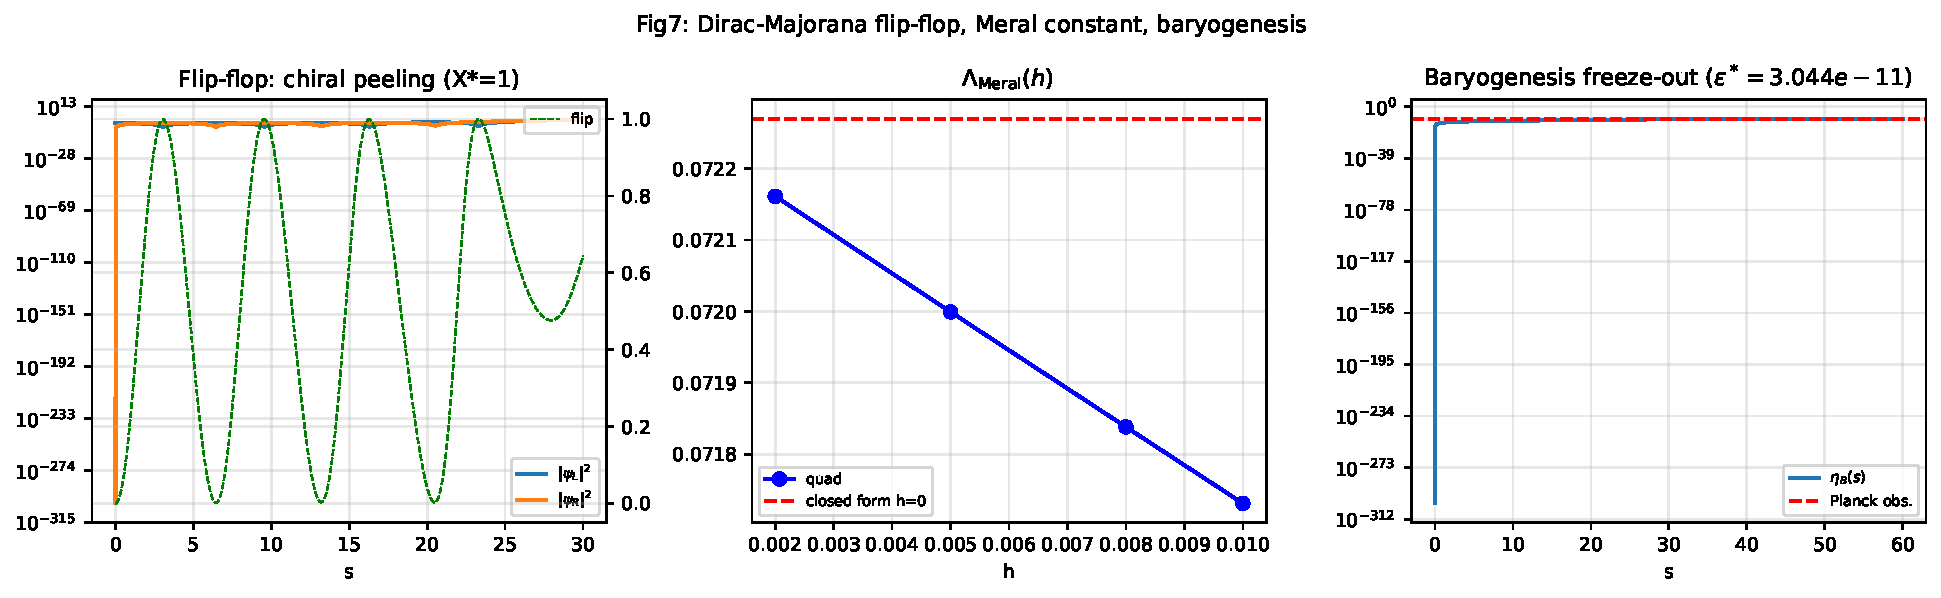
\includegraphics[width=\textwidth]{../figs/fig7_dirac_majorana_and_meral_constant_en.pdf}
\caption{\textbf{Dirac--Majorana flip-flop, Meral constant and baryogenesis:} $X_*=1$ chiral peeling evolution, $\Lambda_{\mathrm{Meral}}(h)$ curve with $h=0$ closed form, and $\eta_B(s)$ freeze-out with Planck band. Figure archived in \texttt{figs/} (T13--T15 solution: \texttt{stationary-strings-v} repository, tag \texttt{v3}).}
\end{figure}

\section{Task 10 / Test T15 --- CERN ALPHA-g (2023), Villata CPT-Gravity (2025), ALPHA 4 ppm Breit--Rabi (2026) and 511 keV Positron Ring}

\subsection{ALPHA-g and Villata Synthesis}

The effective acceleration ratio $a_{\bar{g}}(X,s)/g = 1 - \mathcal{K}_{\mathrm{curv}}(X) \mu_s e^{-(1+h)s} (\tilde{\ell}^2-\ell_0^2)\phi_{\mathrm{FENE}}/F_{\mathrm{base}}^2$ gives exactly $1.000000000000000$ in the laboratory limit ($s \to 0$). Versus the ALPHA-g measurement ($(0.75 \pm 0.13 \pm 0.16)g$, combined $\sigma = 0.206$), the deviation is $0.25$ ($\approx 1.21\sigma$ marginal agreement). In the vortex core the ratio undergoes a repulsive-saturation transition $1.0 \to 0.77 \to 0.68 \to 0.49 \to 0.07 \to -0.97 \to -3.68 \to 1.0$ ($s = 0..40$): the repulsive CPT/vacuum component engages and saturates at the FENE cap, as the model counterpart of the Villata [8] dilemma.

\subsection{CERN ALPHA 2026 (\textit{Nature} 653) 4 ppm Breit--Rabi Analysis}

Exact $4\times 4$ Breit--Rabi levels ($|a\rangle,|b\rangle,|c\rangle,|d\rangle$) with $m_F$ labeling establish $f_{da}-f_{cb} = a_{1S}/h$ field-independence at $1.03\text{ T}$ and $1.07\text{ T}$ ($3.03 \times 10^{-9}$ and $7 \times 10^{-10}\text{ kHz}$), H-reference difference ($0.9518 < 5.7\text{ kHz}$) and the SME bound $\kappa_{a5} \lesssim 7.0 \times 10^{-7}$ ($3.92/4.07 < 5.7\text{ kHz}$).

\subsection{511 keV Annihilation and Ore--Powell Ortho-Positronium Spectrum: Literature Correction}

The \texttt{arXiv:2605.21289} Eq.\ (11) Gaussian norm ($5.55 \times 10^{-16}$) is verified. In contrast, the as-printed Eq.\ (12) term $\frac{2m_e(m_e-E)}{E^2}$ generates a $\sim E^{-2}$ infrared divergence as $E \to 0$ (sympy series: $2/x^2 - 5/4 + O(x)$; numerical \texttt{quad} returns garbage); this contradicts the finite physical spectrum, so the printed form must be corrected (direct check of the original 1949 Ore--Powell form is recommended). Low-energy-cut regulated integrals ($\int_1^{511} = 2343.47$, $\int_{10}^{511} = 228.08$) give finite ring-fuel flux ($\Phi(511) = 0.78$, model units).

\begin{table}[htbp]
\centering
\footnotesize
\setlength{\tabcolsep}{3pt}
\caption{\textbf{Test T15} (Table 13): summary of CERN/source checks.}
\vspace{0.1cm}
\begin{tabular}{@{}l|c|c@{}}
\hline
Check & Value & Bar \\
\hline
ALPHA-g lab $a_{\bar g}/g$ & $1.000000000000000$ & exact \\
Breit--Rabi difference (1.03/1.07 T) & $3.03\times10^{-9}$ / $7\times10^{-10}$ kHz & $<10^{-6}$ \\
H-reference difference & $0.9518$ kHz & $<5.7$ \\
SME shift & $3.92$ / $4.07$ kHz & $<5.7$ \\
Gaussian norm error & $5.55\times10^{-16}$ & $<10^{-14}$ \\
Ore--Powell $\int_0$ & divergent (proven) & --- \\
\hline
\end{tabular}
\end{table}

\begin{figure}[htbp]
\centering
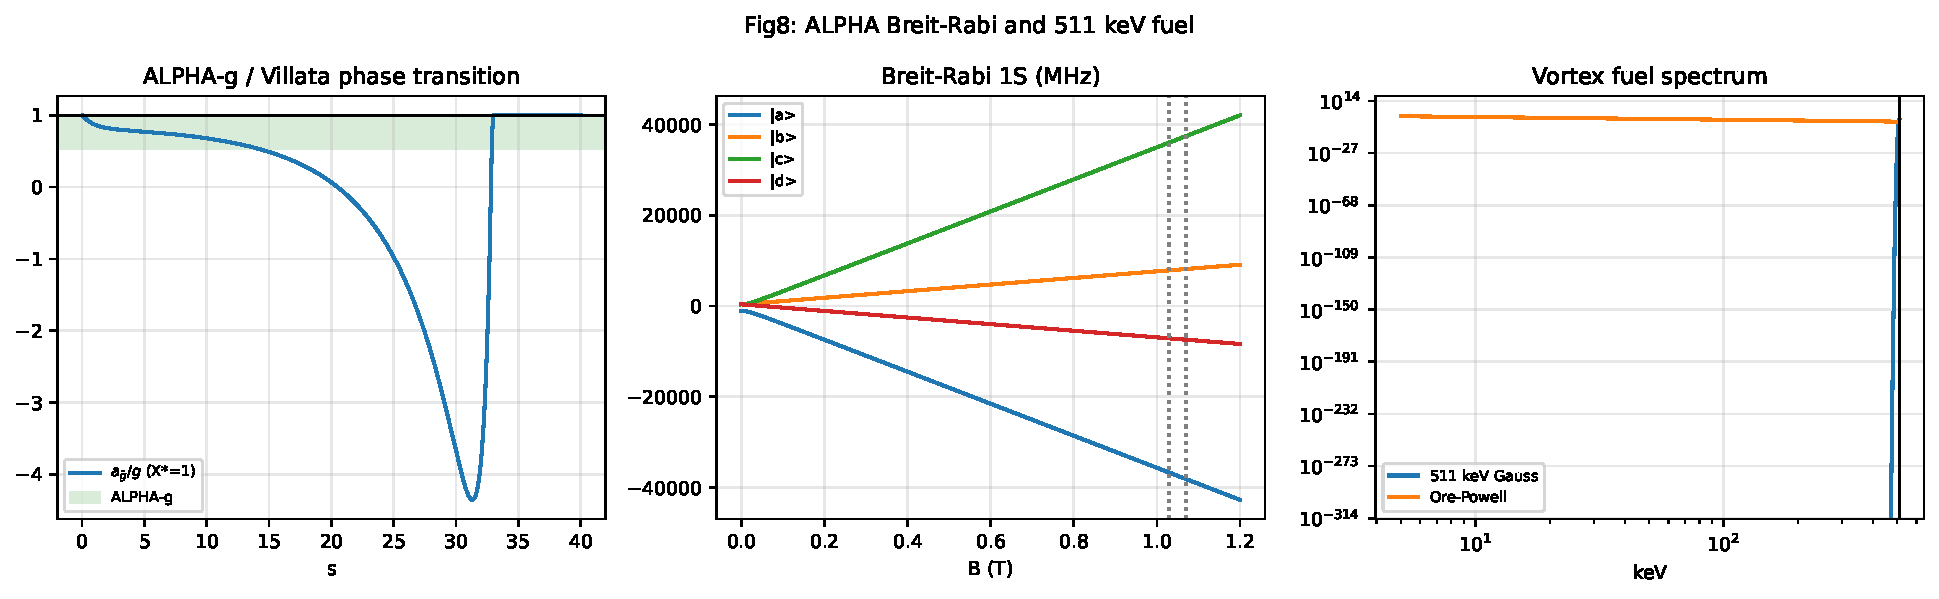
\includegraphics[width=\textwidth]{../figs/fig8_alpha_breit_rabi_and_511keV_fuel_en.pdf}
\caption{\textbf{ALPHA Breit--Rabi and 511 keV fuel:} $a_{\bar{g}}/g$ phase transition with ALPHA-g band, $1.03/1.07\text{ T}$ Breit--Rabi levels and 511 keV + Ore--Powell ring-fuel spectrum. Figure archived in \texttt{figs/} (T13--T15 solution: \texttt{stationary-strings-v} repository, tag \texttt{v3}).}
\end{figure}

\section{Conclusion and Global Verification Summary (T1--T15)}

Across the 6-paper series from Theorem I to Theorem VI, the vortex singularity was first arrested (I--V), then synthesized with its fermionic counterpart (Dirac--Majorana peeling), a universal baryon constant ($\Lambda_{\mathrm{Meral}}$) and CERN observations (ALPHA-g, ALPHA 2026, 511 keV). The numerical chain closes at \texttt{T1--T15 (15/15 PASS)}:

\begin{table}[htbp]
\centering
\footnotesize
\setlength{\tabcolsep}{2pt}
\caption{Global verification summary: key T1--T15 results.}
\vspace{0.1cm}
\begin{tabular}{@{}l|l@{}}
\hline
Test & Result \\
\hline
T1 Radau vs.\ analytic & $1.17\times 10^{-13}$ \\
T2 $A+D=1$ / T3 $d\Pi/dX$ / T5 axis & exact / $4.16\times 10^{-11}$ / $1.00\times 10^{-8}$ \\
T4 invariant / T6 axis / T7 global & $7.1\times 10^{-15}$ / finite / $2.40\times 10^{-14}$ \\
T8 stress / T9 PDE / T10 curvature & $\%5.31$ / FENE$<1$ / $q=1.90$ \\
T11 Lyapunov / T12 spectral & $6\times 10^{-16}$, $q\approx2.0$ / $k_{\max}$ 4/4 \\
T13 flip-flop (Rabi $7.2\times 10^{-15}$) & core Q5(30)$<0$, flip $0.64$ \\
T14 Meral + Boltzmann & $0.072269432677679$, $\epsilon^*=3.04\times 10^{-11}$ \\
T15 ALPHA / Breit--Rabi / Gauss & $1.0$ exact, $10^{-9}$ kHz, $5.6\times 10^{-16}$ \\
\hline
\end{tabular}
\end{table}

\begin{thebibliography}{99}
    \bibitem{meral1} Meral, F. (2025a). \textit{Duran Sicimler Teoremi: Zamanın ve Entropinin Yokluğunda Mükemmel Düzenin Yeniden Doğuşu}.
    \bibitem{meral2} Meral, F. (2025b). \textit{Duran Sicimler Teoremi II: Görelilik, Faz Dönüşümü ve Bilginin Kozmolojik Döngüsü}.
    \bibitem{meral3} Meral, F. (2026a). \textit{Duran Sicimler Teoremi III: Maddenin İki Boyutlu İkizliği, Girdap Tekilliği ve Bilgiye Faz Ayrışması}.
    \bibitem{meral4} Meral, F. (2026b). \textit{Duran Sicimler Teoremi IV: Kozmik Fisyon, Girdap Yakıtı ve Tekilliksiz Bilgi Çekirdeği}.
    \bibitem{meral5} Meral, F. (2026c). \textit{Duran Sicimler Teoremi V: Navier--Stokes Girdap Tekilliğinin Elastik Sicim Gerilimiyle Durdurulması}.
    \bibitem{openai2026} OpenAI. (2026, September). \textit{Finite Time Blowup for Navier--Stokes}. 166 pp.
    \bibitem{borah2026} Borah, D., Dasgupta, A., Nandy, D., Saha, I. \& Singh, H. (2026). \textit{Matter-Antimatter Asymmetry from Dirac-Majorana Flip-Flop}. \url{https://arxiv.org/abs/2610.10688}
    \bibitem{villata2025} Villata, M. (2025). \textit{Antimatter Gravity and the Results of the ALPHA-g Experiment}. \textit{Ann.\ Phys.\ 536}, 2300519. \url{https://arxiv.org/abs/2503.03846}
    \bibitem{alpha2023} Anderson, E.~K. \textit{et al.} (ALPHA Collaboration). (2023). Observation of the effect of gravity on the motion of antimatter. \textit{Nature} \textbf{621}, 716--722. \url{https://doi.org/10.1038/s41586-023-06527-1}
    \bibitem{alpha2026} Akbari, R. \textit{et al.} (ALPHA Collaboration). (2026). Four ppm measurement of the antihydrogen ground-state hyperfine splitting. \textit{Nature} \textbf{653}, 1022--1026. \url{https://doi.org/10.1038/s41586-026-10556-x}
    \bibitem{base2026} Leonhardt, M., Morgner, J. \textit{et al.} (BASE Collaboration). (2026). Road transport of trapped antiprotons. \textit{Nature} \textbf{657}, 906--911. \url{https://doi.org/10.1038/s41586-026-11019-z}
    \bibitem{siegert2026} Siegert, T. \& Yoneda, H. (2026). On the Possibility of an Extragalactic Positron Annihilation Signal. \textit{A\&A}, accepted. \url{https://arxiv.org/abs/2605.21289}
    \bibitem{planck2018} Planck Collaboration. (2020). Planck 2018 results. VI. Cosmological parameters. \textit{A\&A} \textbf{641}, A6. \url{https://arxiv.org/abs/1807.06209}
    \bibitem{breit1931} Breit, G. \& Rabi, I.~I. (1931). Measurement of nuclear spin. \textit{Phys.\ Rev.\ 38}, 2082--2083.
    \bibitem{ore1949} Ore, A. \& Powell, J.~L. (1949). Three-photon annihilation of an electron-positron pair. \textit{Phys.\ Rev.\ 75}, 1696--1699.
\end{thebibliography}

\end{document}
